\chapter{Literature Survey}

We searched for various papers related to machine learning, classification and labelling of text sections related to a topic. Considering as this is a field with a lot of ongoing research and work, we found a fair few number of published papers which we read to gain an insight into the approach that we will follow.\\

Teevan et al.\cite{teevan} have discussed the relevance of using search methodologies that focus more on contextual information as opposed to simple keyword matching as that may not be enough the capture the relevant text. 

Joachims has also concluded\cite{joachims} that SVMs are an effective text classification tool which uses the Supervised Machine Learning model. 

Inoue et al.\cite{squint} proposes an SVM based approach to identify the most relevant section in Web pages returned by a search query (SQUINT) and provides an architectural overview of the same. To accomplish this it uses a feature set generated by the Supervised Learning model. \\

We explore a similar architecture to SQUINT in order to have a machine learning approach to extracting questions based on topics from web pages.

\chapter{Design}

We have settled on a component---based architecture for the application which we believe will be feasible to implement. 

Having a component based architecture is suitable for this application because each component has a well defined function which is more-or-less independent of the other sections. 
This will help in having a de-coupled structure and each component can be modified without affecting the other components. 

\section{Components}

The high---level view of the architecture is as follows : 

\begin{center}
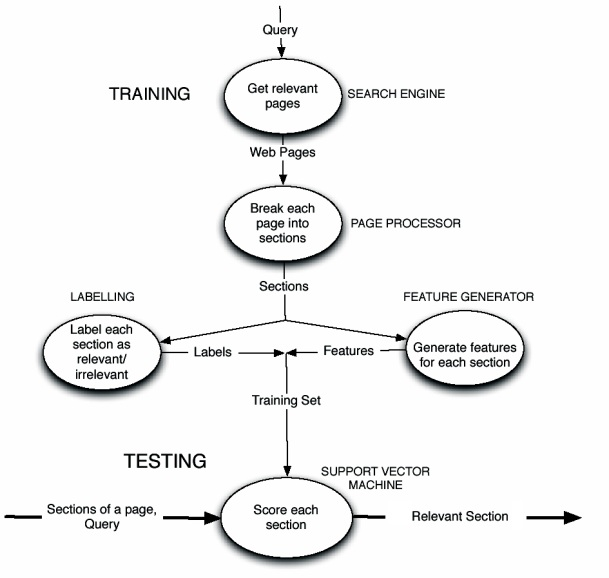
\includegraphics[width=0.80\textwidth]{./architecture}\\
\end{center}

\subsection{Query}

Firstly, we will take the input of the topic and generate a list of sub-topics and other keywords which relate to the topic. For eg. if the topic is ``Operating Systems", various sub-topics can be ``Processes", ``Threads", "Memory Management" etc.

This list of keywords will then be used to generate a number of key--phrases comprising set Q which will be queried on the search engine to get a list of pages which are likely to contain questions related to the required topic. These pages will comprise the set P.

\subsection{Page Preprocessor}

Each page that we load will need to be stripped of all useless markup data, links and pictures and we need to parse out only the text portions available on the page which may contain the questions. 

The page will then be broken into various sections which will be passed onto the further components.

The set S will contain all sections from all pages that we have loaded: 

\textit{S = \{s; s is a section in some page in P\}}

\subsection{Feature Generator}

The feature generator will generate the features and statistics for each section, which will be analysed by the SVM to create the regression model, based on the following : 

\begin{itemize}
	\item Word Rank Based Features
	\item Bigram Rank Based Features
	\item Coverage of Top Ranked Tokens
	\item Distance from the Query
	\item Query Word Frequency
\end{itemize}

\subsection{Labelling}

For generating the training set, we will manually label a set of sections as to whether they are relevant questions of the given topic or not and this data will be used by the SVM to generate the model. The difficulty level of the question will also be given a rating on a scale of 10.

\subsection{Support Vector Machine}

The Support Vector Machine component will be trained using the Training Set comprising of the section set with the generated features and manually tagged labels. 

This will use the data to generate a regression model. \\

This will then be used to identify the relevant questions sections and will also assign them a difficulty rating. \\

The SVM based approach to identify the most relevant section in a web--page (SQUINT) \cite{squint} was developed to deal with big sections of text but can be adapted to our use--case by tweaking the feature-set parameters. 

\subsection{Output}

The output component will take all the questions extracted and output them in a clean format sorted on the basis of difficulty.

\section{Programming Language}

With regards to programming language in which we will implement the project, we have narrowed down the choices to the following : 
\begin{description}
	\item[Java] A very popular Object Oriented Language with lots of packages available for most algorithms and data structures.
	\item[Octave] An interpreted language with support for Machine Learning models.
\end{description}

\chapter{Further Work}

While the overall architecture of the application seems promising, each component needs to be designed with an elaborate algorithm and appropriate data structures need to be chosen after detailed analysis. \\

We will continue to follow the latest research related to machine learning in order to tune the machine learning algorithm which will identify questions. \\

Once the design is finalised, we plan to start the basic implementation of the application and hope to achieve significant progress on at least 1 component by the end of this semester.

